The classification of unlabelled data is completed using the code presented in
Section \ref{sec:q5}. MATLAB actually provides a number of built in functions
for classifying data by k-means and fuzzy k-means
which are used extensively in this implementation.

MATLAB's \texttt{kmeans} and \texttt{fcm} functions are used to cluster the
provided data. Much of the remainder of the code in Section \ref{sec:q5} is
devoted to creating the plots in Figures \ref{fig:k-means-clear}, \ref{fig:k-means-multifuzz} and \ref{fig:k-means-gradientfuzz}.

\begin{figure}
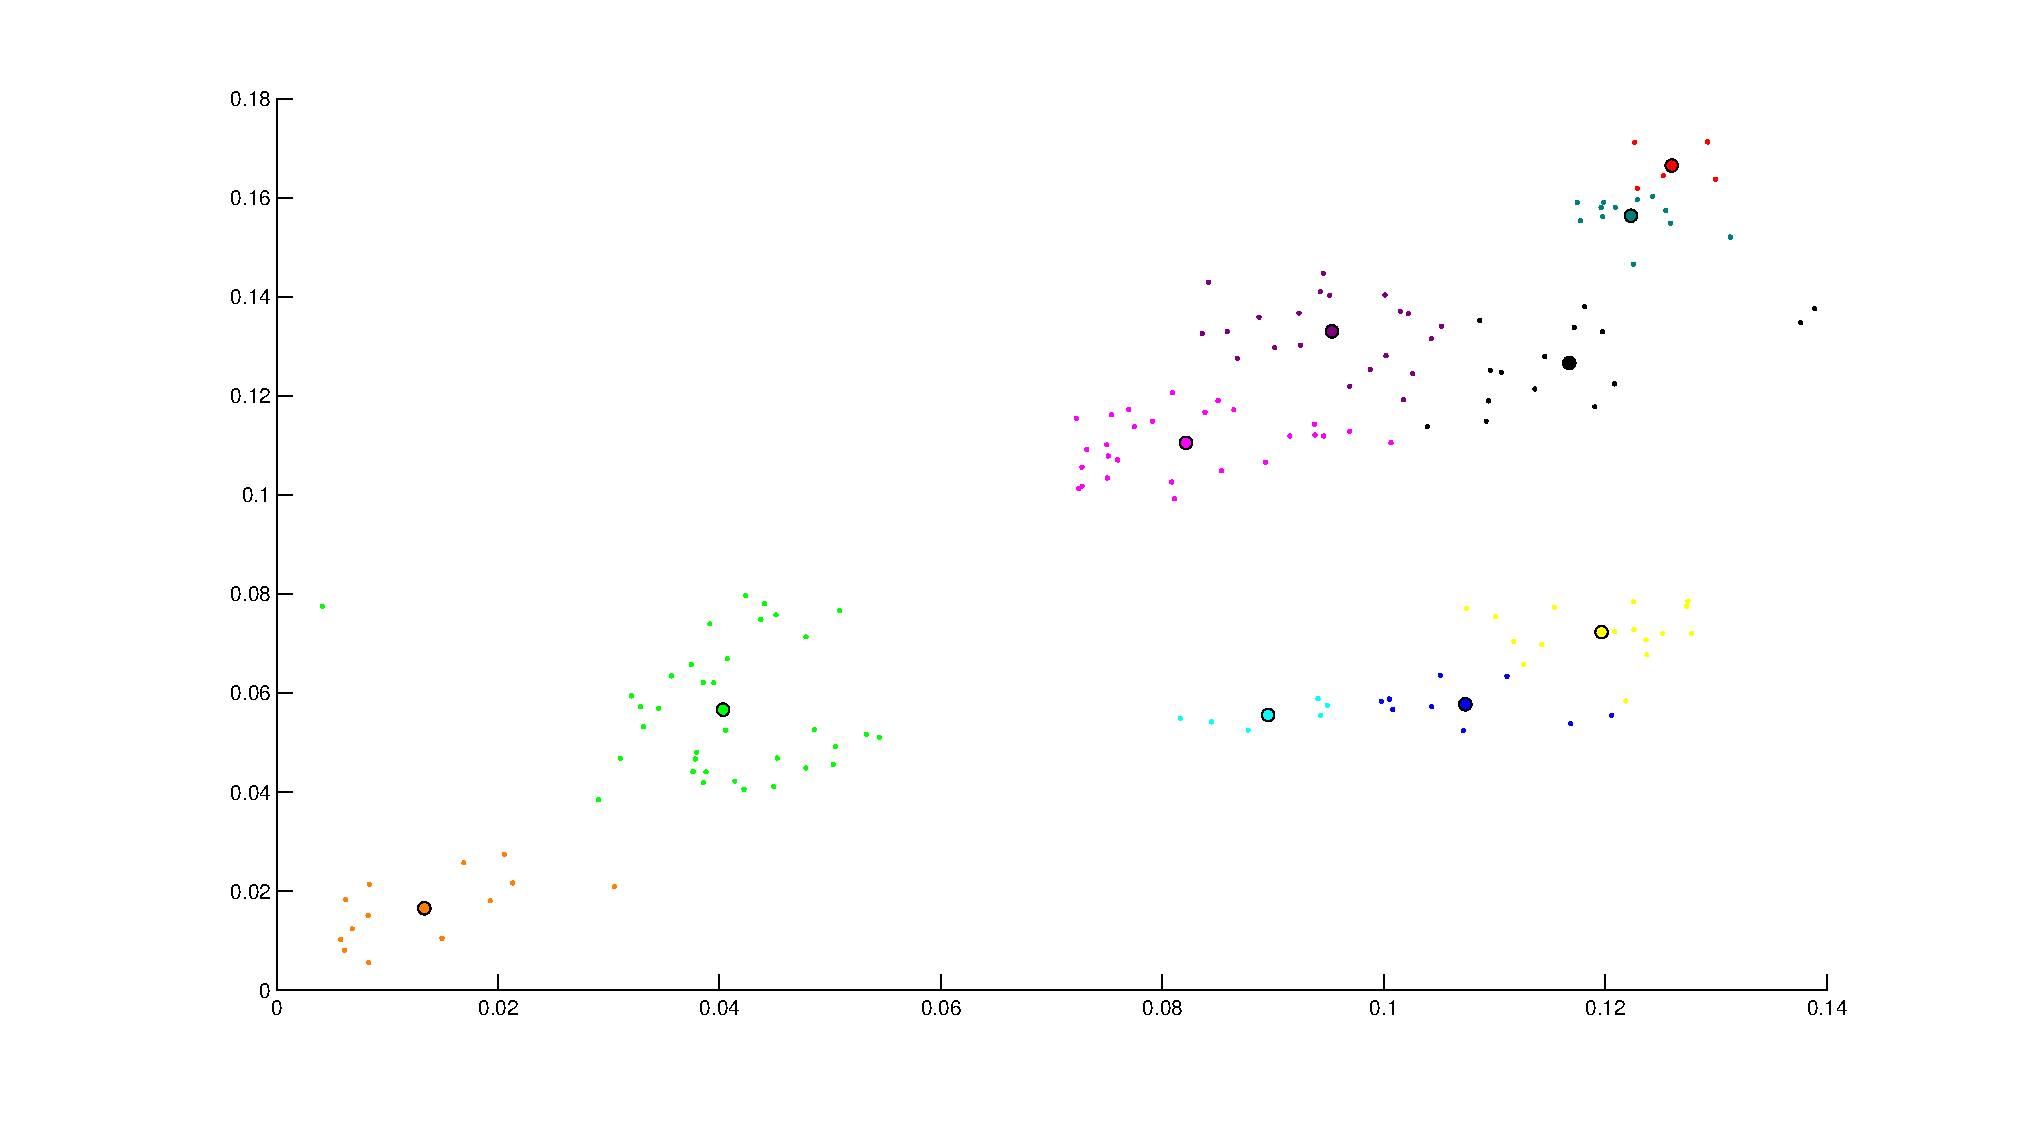
\includegraphics[width=\textwidth]{images/clear-coloured}
\label{fig:k-means-clear}
\caption{K-means clusters, colour-coded with prototypes outlined in black}
\end{figure}

\begin{figure}
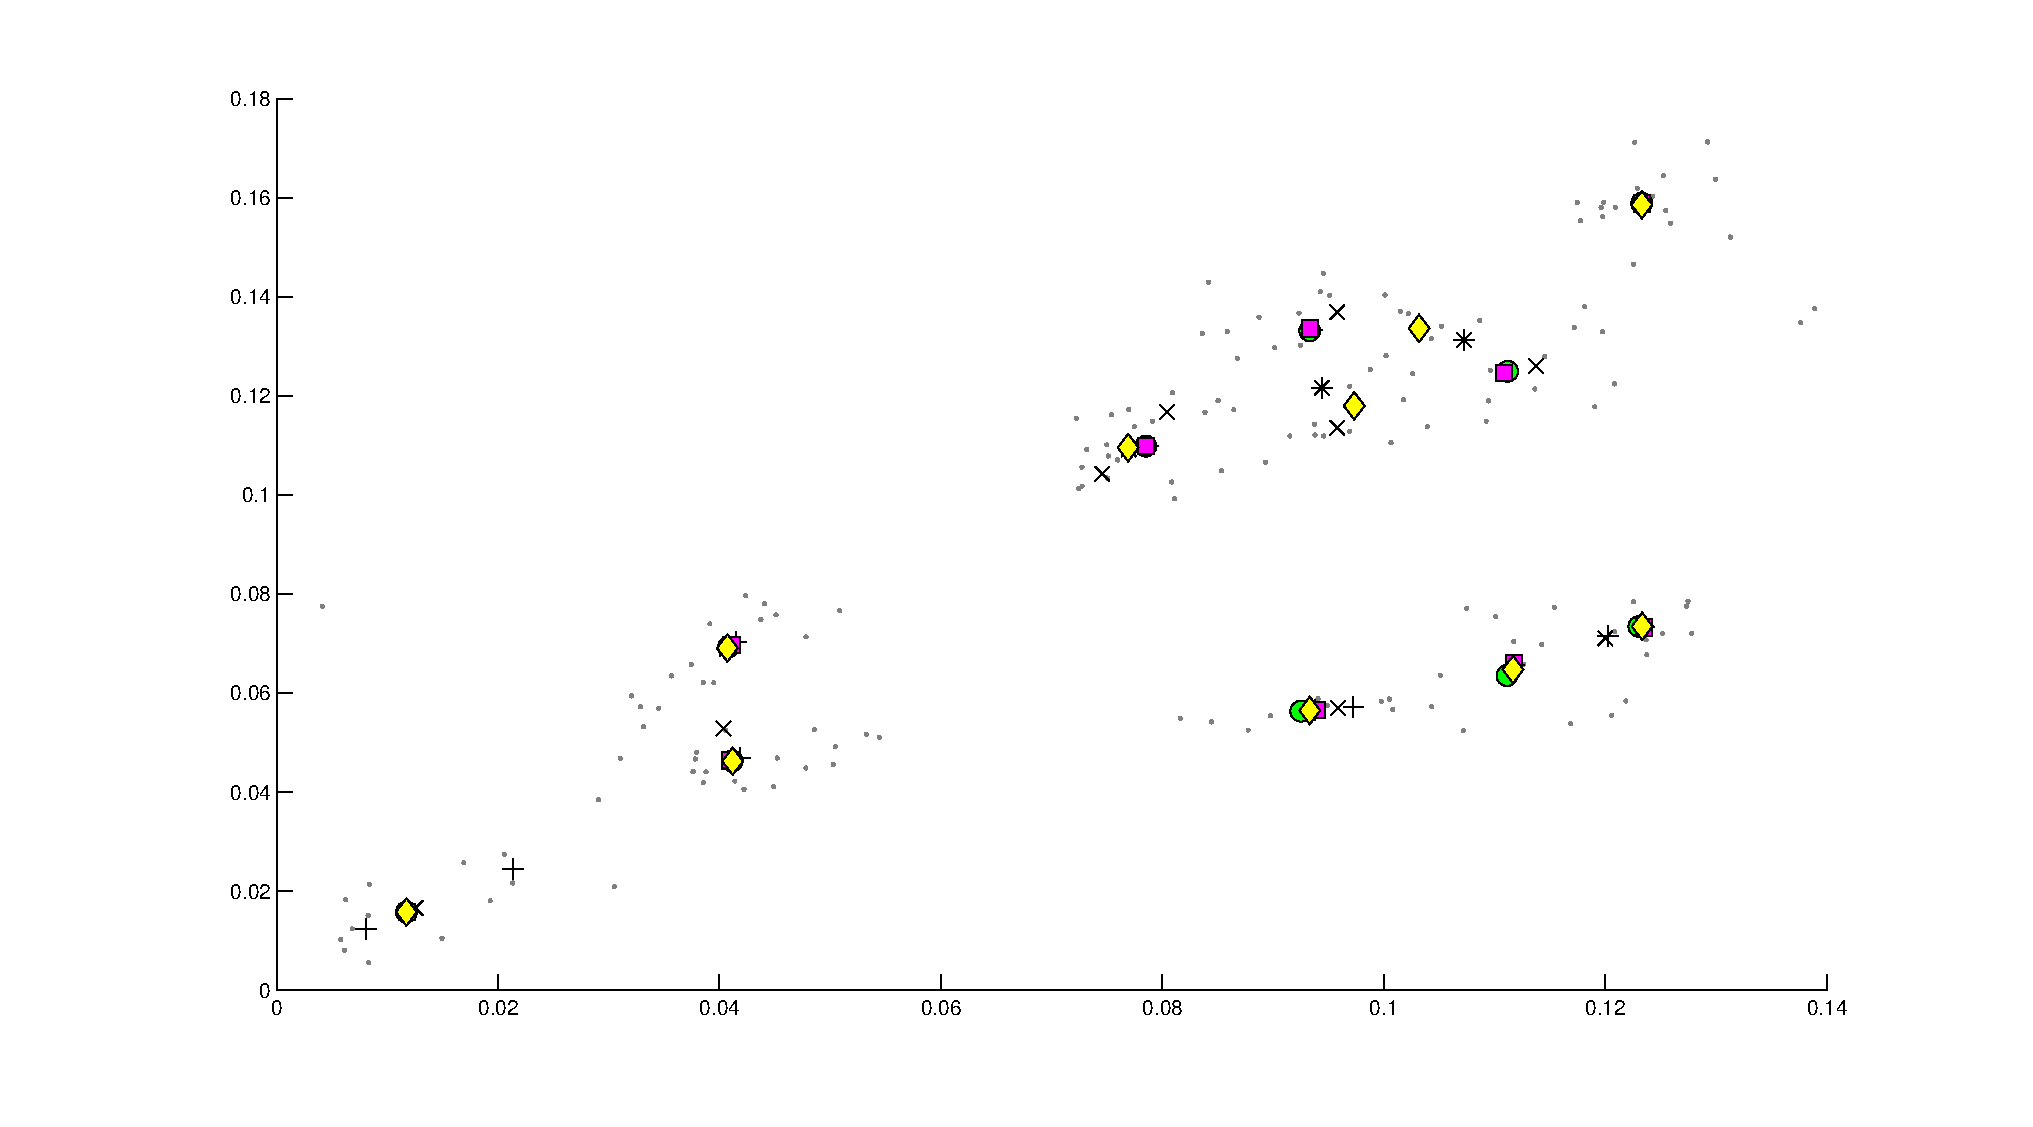
\includegraphics[width=\textwidth]{images/fuzzy-multiple}
\label{fig:k-means-multifuzz}
\caption{Prototypes from multiple runs of the k-means clustering algorithm
(distinct prototype shape and colour for each run)}
\end{figure}

\begin{figure}
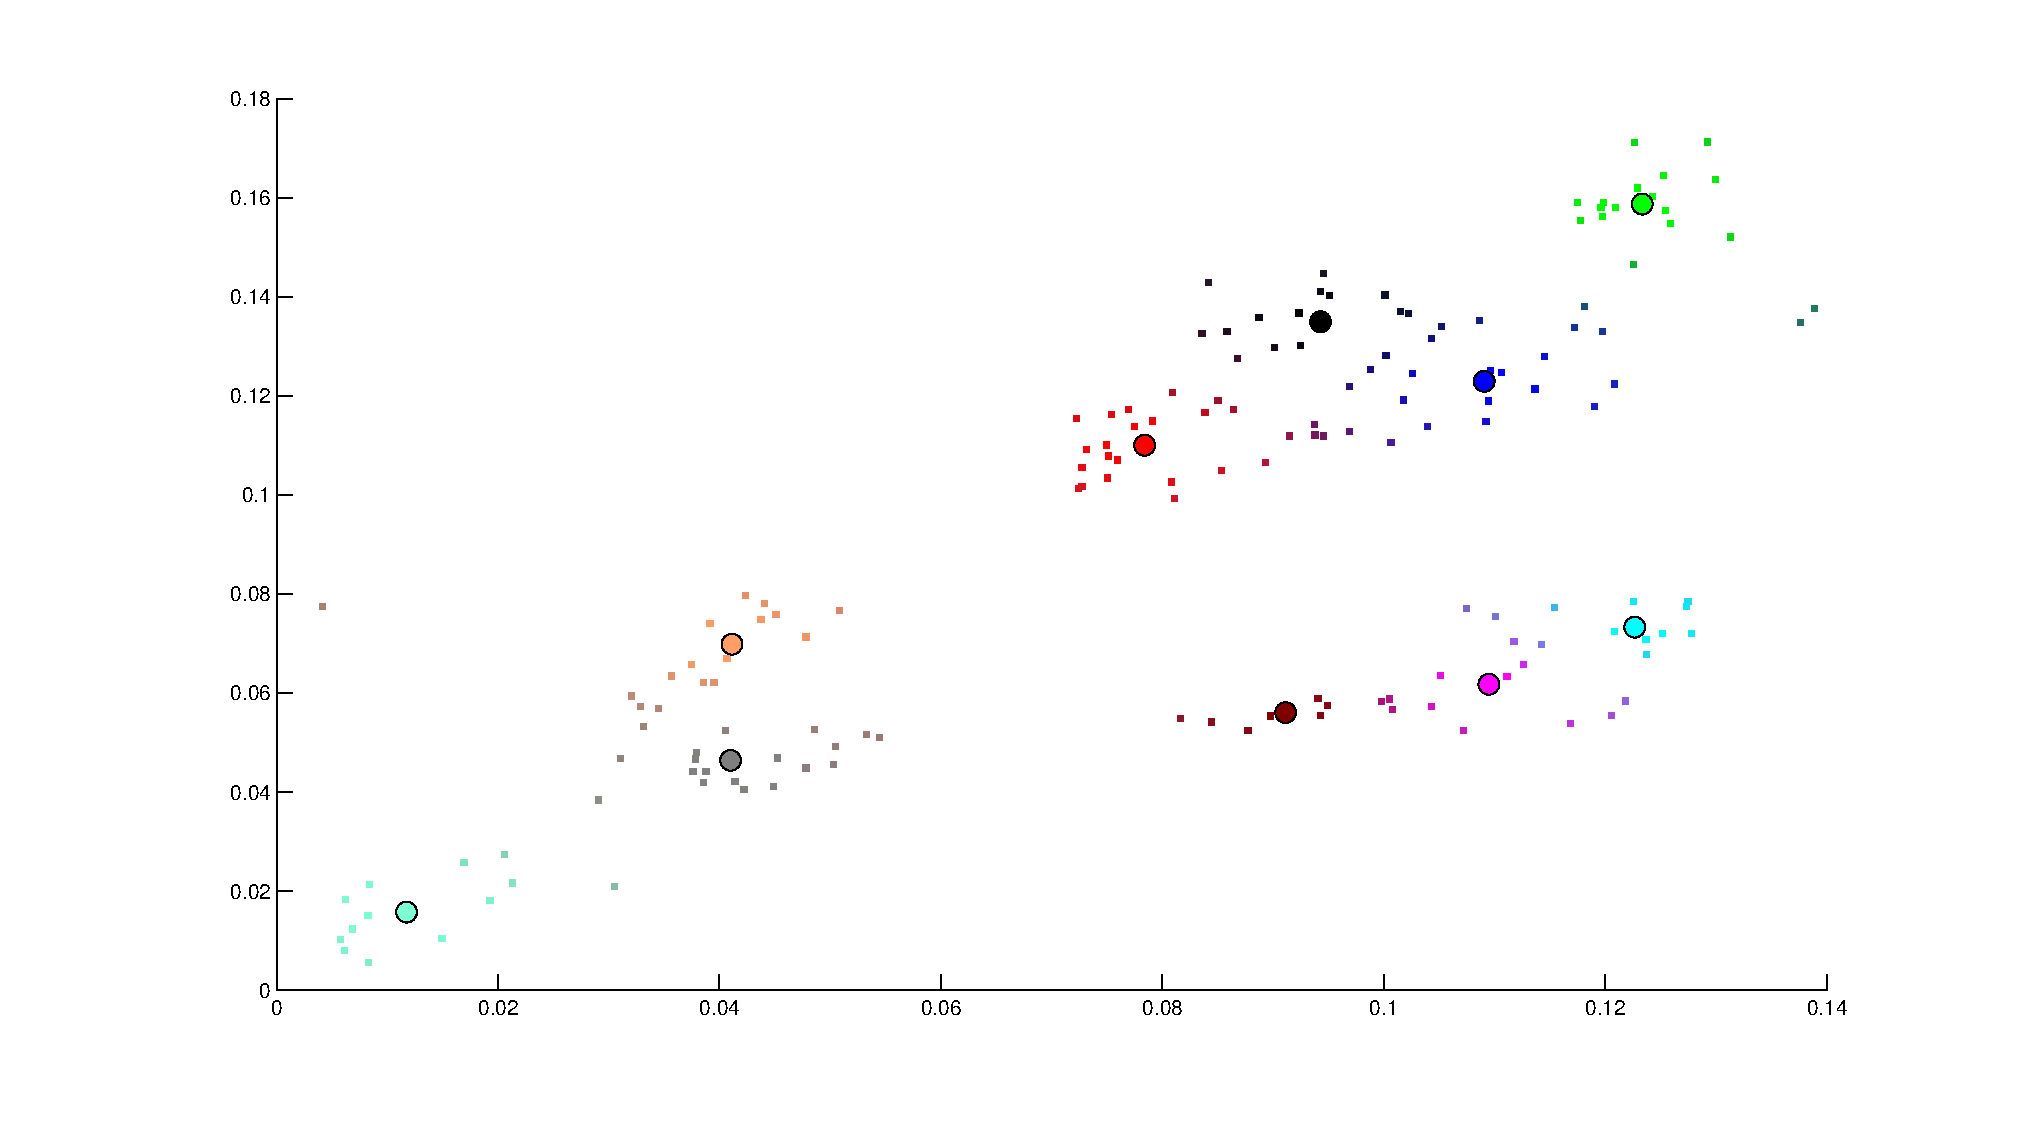
\includegraphics[width=\textwidth]{images/fuzzy-gradient}
\label{fig:k-means-gradientfuzz}
\caption{Prototypes from fuzzy k-means clusters. Data points are
shaded based on probability of belonging to a cluster.}
\end{figure}